\documentclass{article}
\usepackage{graphicx}
\usepackage[margin=1.5cm]{geometry}
\usepackage{amsmath}

\begin{document}
\twocolumn

\title{Tuesday Warm Up, Unit 1: Filter Design}
\author{Prof. Jordan C. Hanson}
\maketitle

\section{Memory Bank}

\begin{enumerate}
\item \textbf{Note:} in the following formulas, $f_{\rm C}$ is taken to be a fraction of the sampling frequency, so it has no units.
\item \textbf{The sinc function} is the inverse DFT of the ideal low-pass filter in the frequency-domain:
\begin{equation}
h[i] = \sin(2\pi f_{\rm C}i)/(i\pi)
\end{equation}
For $i\to 0$, $h[i] \to 2$.  The sinc function is usually defined over $M$ samples, shifted right by $M/2$ samples.
\item \textbf{The Blackman window} is a window for a filter kernel like the sinc function, to remove unwanted effects due to the finite length of $h[i]$.
\begin{equation}
w[i] = 0.42 - 0.5\cos(2\pi i/M)+0.08\cos(4\pi i/M)
\end{equation}
\item \textbf{The windowed-sinc filter} is the product of the sinc kernel and the Blackman window:
\begin{equation}
h[i] = K \left(\frac{\sin(2\pi f_{\rm C}(i-M/2))}{i-M/2}\right)w[i] \label{eq:1}
\end{equation}
The factor $K$ must be set so that the sum of all the samples must be 1.  For $i=M/2$, $h[i] = 2\pi f_{\rm C} K$.
\item \textbf{The convolution theorem} states that the Fourier transform of the convolution of two functions is the same as the product of the Fourier transforms of the two functions.
\end{enumerate}

\section{Windowed-Sinc Filters}

\begin{enumerate}
\item Write octave functions that (a) implement the sinc function, and (b) implement the Blackman window.
\item Write an octave function that implements the product of the sinc and Blackman window, following Eq. \ref{eq:1}.
\item Using the \verb+octave+ function \verb+sum+, compute the sum of the samples in your filter kernel, given $M$ and $f_{\rm C}$.  Set $K$ equal to the reciprocal of the result, so your windowed-sinc function is \textit{normalized.}  That is, the sum of the samples in the kernel is set to 1.
\item Generate a vector of white noise using \verb+randn+ in the usual way, and convolve it with a kernel output from your windowed-sinc function.
\item (a) Measure the \textit{stop-band attenuation} of your filter.  That is, what is the ratio of attenuated to unattenuated amplitude in the power spectrum? (b) Measure the \textit{roll-off} of your filter.  That is, in how many Hz does the frequency response go from maximum to minimum?
\end{enumerate}

\begin{figure}
\centering
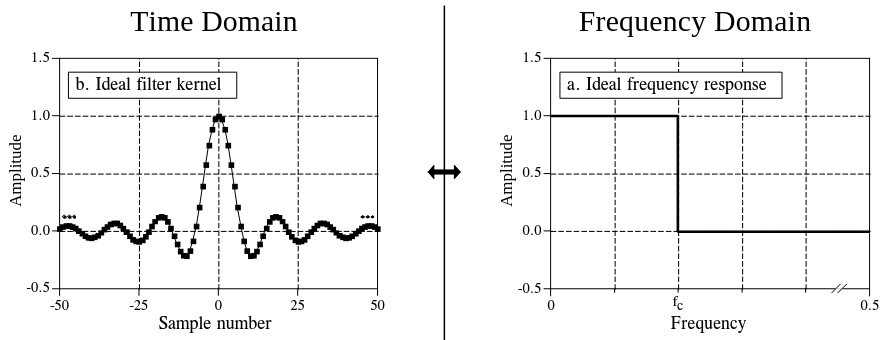
\includegraphics[width=0.5\textwidth]{sinc_filter.png}
\caption{\label{fig:1} The ideal low-pass filter (right) is unattainable, due to the finite nature of the digital sinc function (left).}
\end{figure}

\section{FFT Convolution}

\begin{enumerate}
\item Suppose we are working with a moving-average filter, to remove high-frequency noise.  Our incoming signal is a square wave.  In order to predict the signal output, we must calculate the convolution of a square pulse with a square wave.  Think conceptually about how convolution works.  Show graphically that the convolution of two square pulses should be a triangle wave. \\ \vspace{3cm}
\item One of the fastest ways to convolve two functions is to compute the product of their DFTs, and then compute the inverse DFT of the result.  This algorithm relies on the \textit{convolution theorem.}  Write a short \verb+octave+ script that computes the \verb+fft()+ of two square pulses, multiplies them, and then computes the \verb+ifft()+ (inverse DFT) of the result.  Graph the result to show that it is indeed a triangle wave.
\end{enumerate}

\end{document}
